%!TEX program = xelatex
%!BIB program = bibtex

\documentclass[cn,black,12pt,normal]{elegantnote}
\usepackage{float}
\usepackage{hyperref}

\newcommand{\upcite}[1]{\textsuperscript{\textsuperscript{\cite{#1}}}}

\title{课堂作业\\Lecture 5}
\author{姜文渊\\1951510}
\institute{School of Life Science, Tongji University}
%\version{1.00}
\date{2021年3月26日}

\begin{document}

\maketitle


\section{问题}
\subsection*{问:}

\textit{Try Swiss institute of bioinformatics.}

\subsection*{答:}

\subsection{ExPASy}
\textit{Expasy is the bioinformatics resource portal of the SIB Swiss Institute of Bioinformatics.}

\textit{It is an extensible and integrative portal which provides access to over 160 databases and software tools, developed by SIB Groups and supporting a range of life science and clinical research domains, from genomics, proteomics and structural biology, to evolution and phylogeny, systems biology and medical chemistry.}
\upcite{gasteiger2003expasy}

\begin{figure}[H]
    \centering
    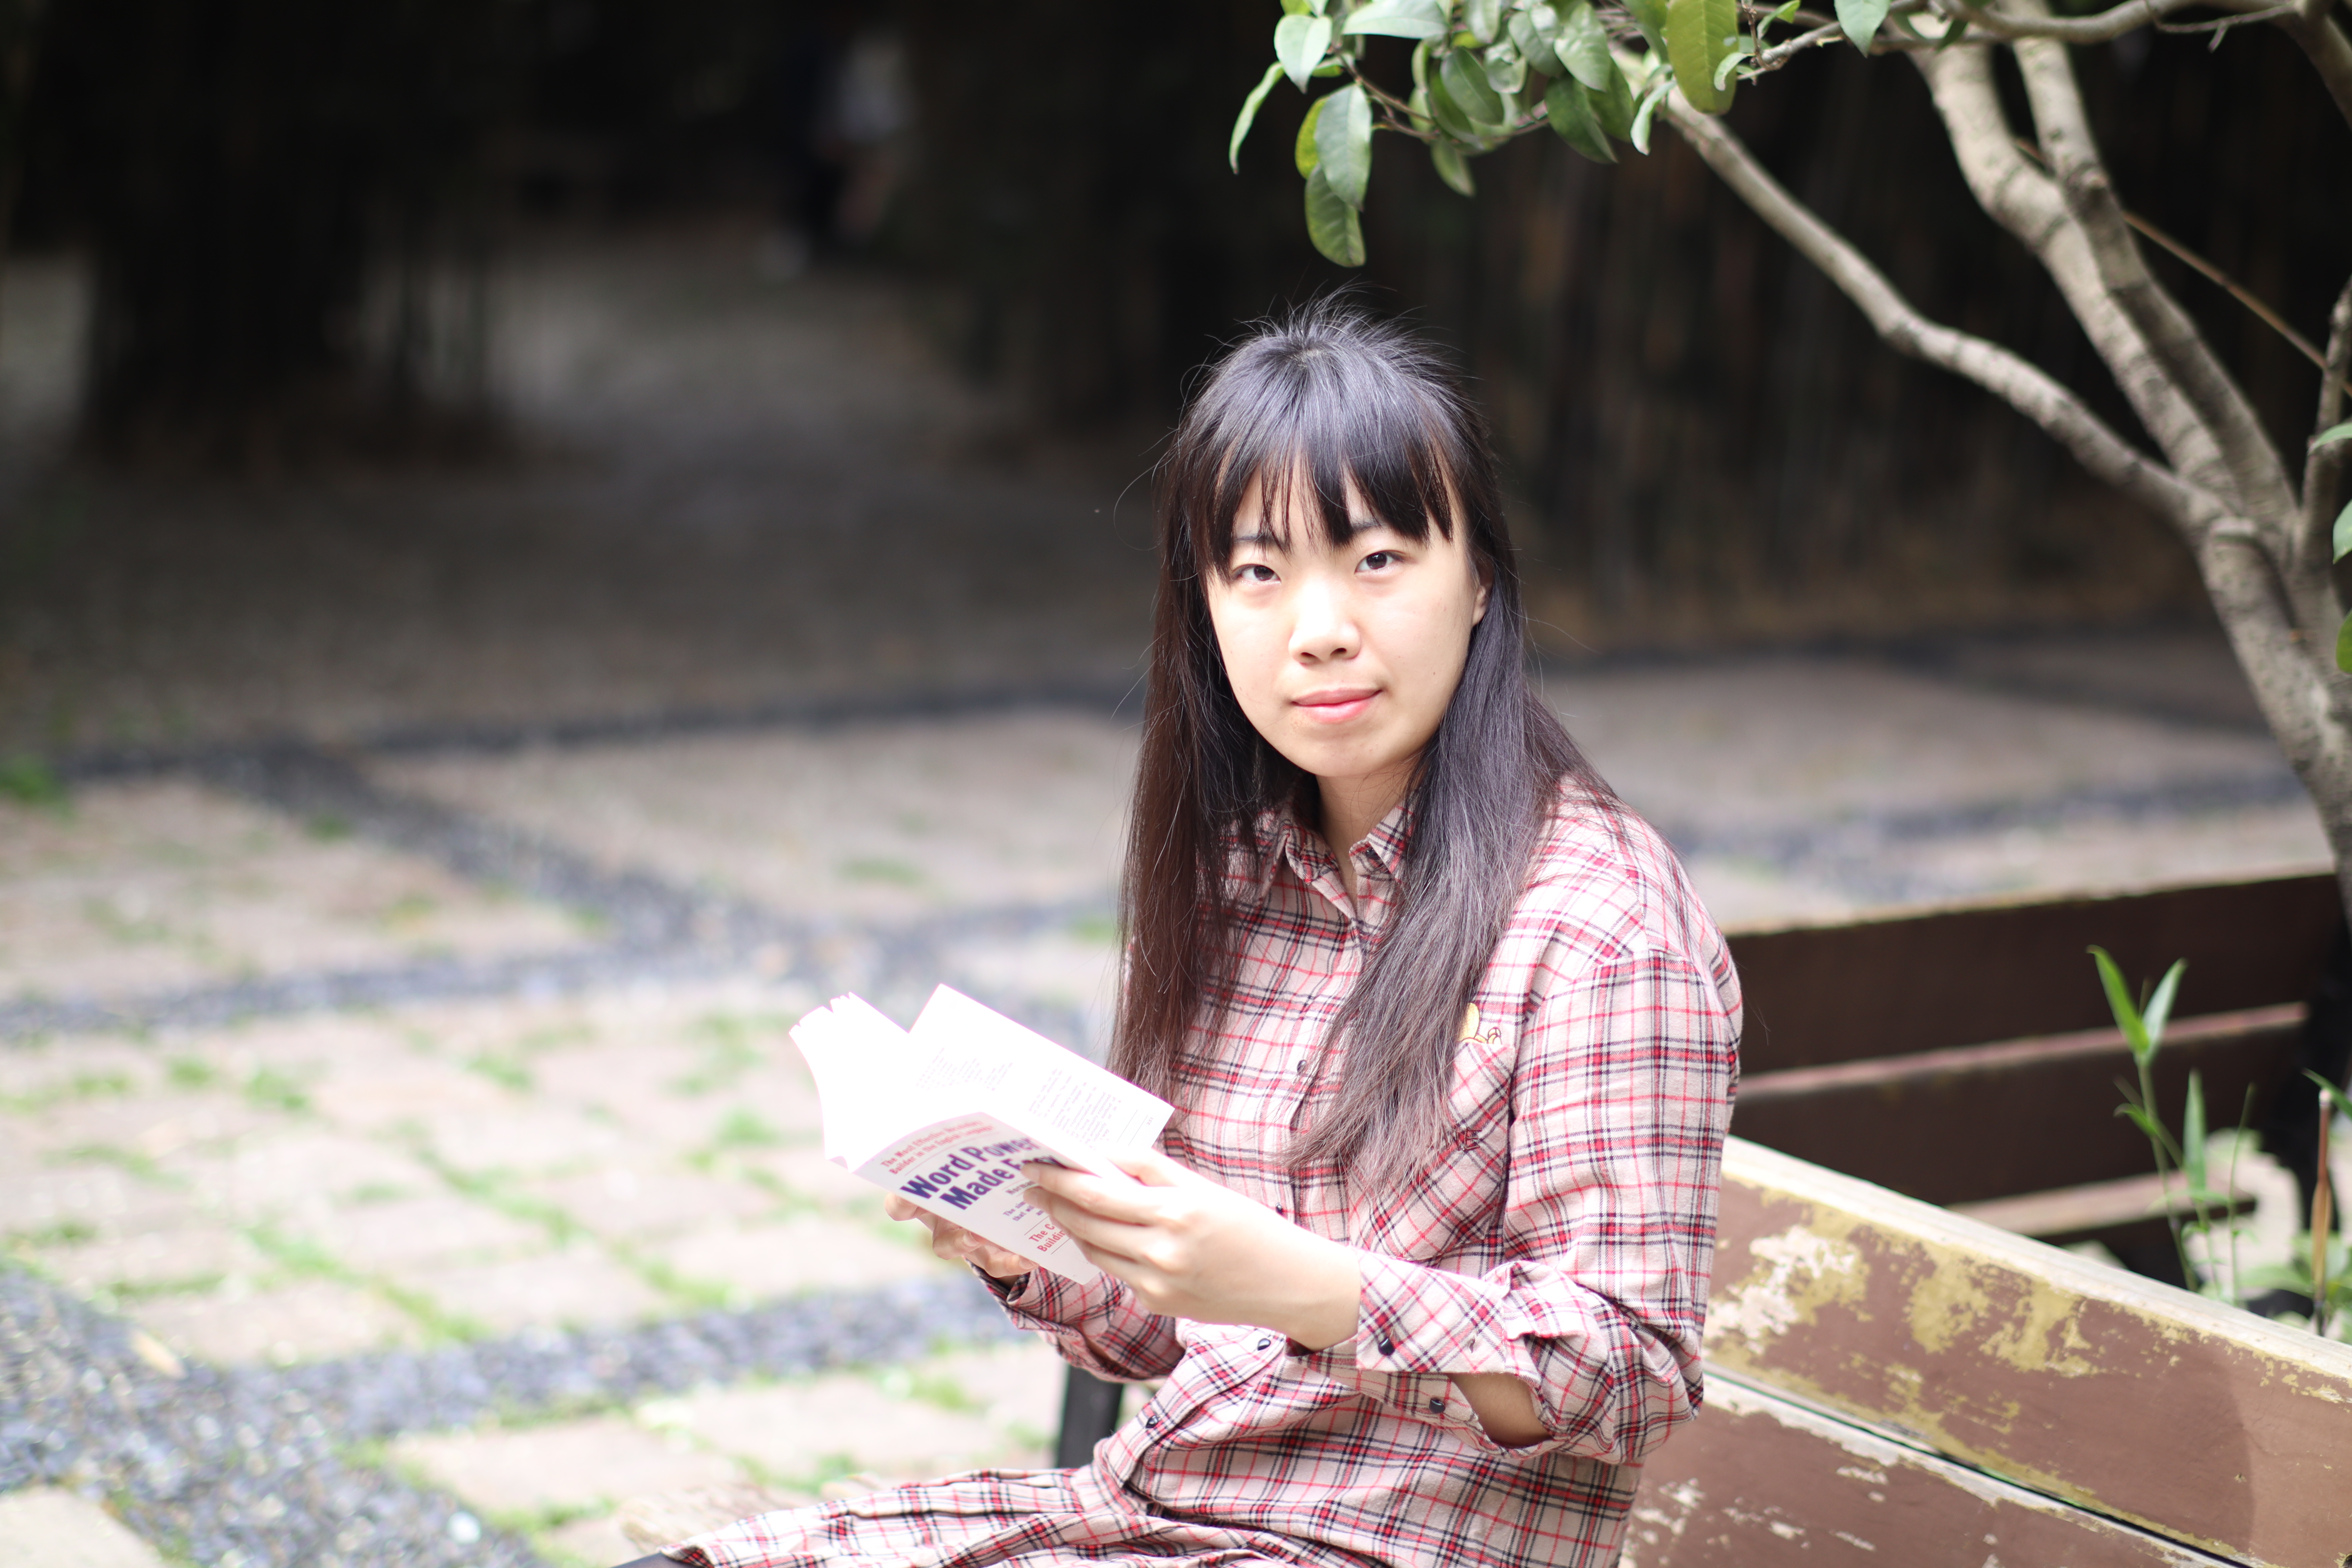
\includegraphics[width=0.7\textwidth]{F1}
    \caption{Home page of ExPASy, retrived on Mar 26 2021.}
    \label{F-01}
\end{figure}

\subsection{UniProt}
\textit{The Universal Protein Resource (UniProt) is a comprehensive resource for protein sequence and annotation data. The UniProt databases are the UniProt Knowledgebase (UniProtKB), the UniProt Reference Clusters (UniRef), and the UniProt Archive (UniParc). The UniProt consortium and host institutions EMBL-EBI, SIB and PIR are committed to the long-term preservation of the UniProt databases.}
\upcite{uniprot2019uniprot}


\section{问题}
\subsection*{问:}

\textit{How to calculate theoretical MW/PI from protein sequence?}

\subsection*{答:}

\bibstyle{unsrt}
\bibliography{references}{}
\end{document}
